\documentclass{article} 
\usepackage{url,listings,graphicx,hyperref,fullpage,float,fancyref,moreverb}
\restylefloat{table}
\usepackage{hyperref}
\usepackage{url}
\usepackage{multicol}
\usepackage[T1]{fontenc}
\usepackage{subcaption}


\title{Masters Research Topics}
\author{
			Authored By:				\\
			Sifat Sultan	1003289 \\			
	   	}


			
\begin{document}


\maketitle

\tableofcontents

\clearpage

\begin{abstract}
This paper discusses various research topics that are trendy now, topics that looks interesting to me and finally how to propose the topic in a way that will catch the attention of the research funding board.
\end{abstract}

\begin{multicols}{2}
\section{Introduction}
A thesis topics is something that should change my life and not something that was done blindly. It should be worth the pain, patience and sacrifice.Hence, I am writing a paper that will act as a decent preparation before I take my research topics. That said, I am still open to any suggestion that my supervisor will make. 

Below is a checklist for a good research topics. The research that I will undertake...
\begin{itemize}
\item is actually needed in the market.
\item is interesting, possible and the end result is strongly motivating.
\item will get me grant.
\item there is a interested team to work with.
\end{itemize}


By the end of this study, I would like to find the following:
\begin{itemize}
\item a topic that has solid reason to strive for, to get funded and the potential market.
\item powerful, easy and familiar programming language to acheive the task.
\end{itemize}


\section{Software Engineering for Sustainability}
\begin{quotation}
Sustainability are means to manage resources efficiently and \textbf{\textit{reduce}} waste, cost.
\end{quotation}

Research in this field attempts to improve ways software can help reduce waste of food, water, energy, raw materials and so on. As an example, one may consider an app for party organizations which can help in reducing food waste by carefully checking how many people will be present and what type of food will they use. \cite{leicester}.


\begin{figure}[h]
	\centering
		
\includegraphics[width=0.2\textwidth]{images/partyapp.png}
		\caption {A Party App}
	\label{fig:Multimeter}
\end{figure}


\section{Compiler}
\subsection{Compiler and Interpreter}
Compilers turn the code into an executable once and then this executable can be run over and over again with different data whereas an interpreter needs to translate the code every time it is run with data.

\subsection{Semantic Analysis}
Semantic checks consist of many checks that tries to find what each sentence actually \textbf{\textit{mean}}.

\subsubsection{Variable Binding}
Its discusses how the compiler tries to understand what does a certain variable mean which of course is derived from the scope the variable is.

\begin{quotation}
\underline{\textit{Jack}} said \underline{\textit{Jerry}} left \underline{\textbf{his}} assignment at home.

\end{quotation}

Programming languages define strict rules to avoid ambiguities.

\subsubsection{Type Checking}
\begin{quotation}
\underline{\textit{Jack}} left \underline{\textit{her}} homework at home.
\end{quotation}
In this sentence, we can notice there is a mismatch in type, the type ``\textbf{her}''  does not go with  ``\textbf{Jack}''. This is where type checking makes sure that they are two different entity and hence referred separately.


\end{multicols}

%----------------------------
%--------AGRICULTURE---------
%----------------------------


\clearpage
\section{Agricultural}
The first step before designing drones for agriculture is to know what problems do the current farmers face.  Patrick Pearse has listed a few possible issues that appears to be a result of good study conducted by the author, in other words; they don't appear to be random fanciful guesses. 

They following are a list of issues that needs to 

\begin{multicols}{2}

\subsection{Technology Used in Farming}
\subsubsection{Greenhouse Smart Water Monitoring System}

Water usage is not a topic that you can expect in a conversation during dinner, however, it is quite an important conversation for those who are financing a commercial greenhouse and various other people related to this industry.In Canada, the water use by ``\textit{Agriculture, forestry, fishing and hunting}'' is about \textbf{1,769,928} thousand m\textsuperscript{3} \cite{greenhousewatering}. This is where small conservation leads to very big changes.

Civil and Environmental Engineering professor Rupp Carrivau and his collaborator, mechanical engineering professor David Ting has come up with a smart meter that ``measures water by the second''.The data collected from the smart meter will actually help the water supplier supply water efficiently. There is three party who will be benifiting; the owner, supplier and the government.

\paragraph{} 
The owner will have to pay less, the supplier knows exactly how much water each greenhouse will need the next time. The water use varies according to seasons. For instance, in summer there will be more use of water than in winter and hence the rate of water conversation is not the same every month. The issue with the previous systems were that it would predict the water supply based on the water usage of the last month. The water usage was derived from the ``monthly water gauge''.



\subsection{Drones Already Used in Farming}
Drones are already in use


\subsection{How Drones Reduced Cost and Increased Growth}
\end{multicols}


\section{Case Study : Arena Flowers}


\begin{figure}[ht]
\centering
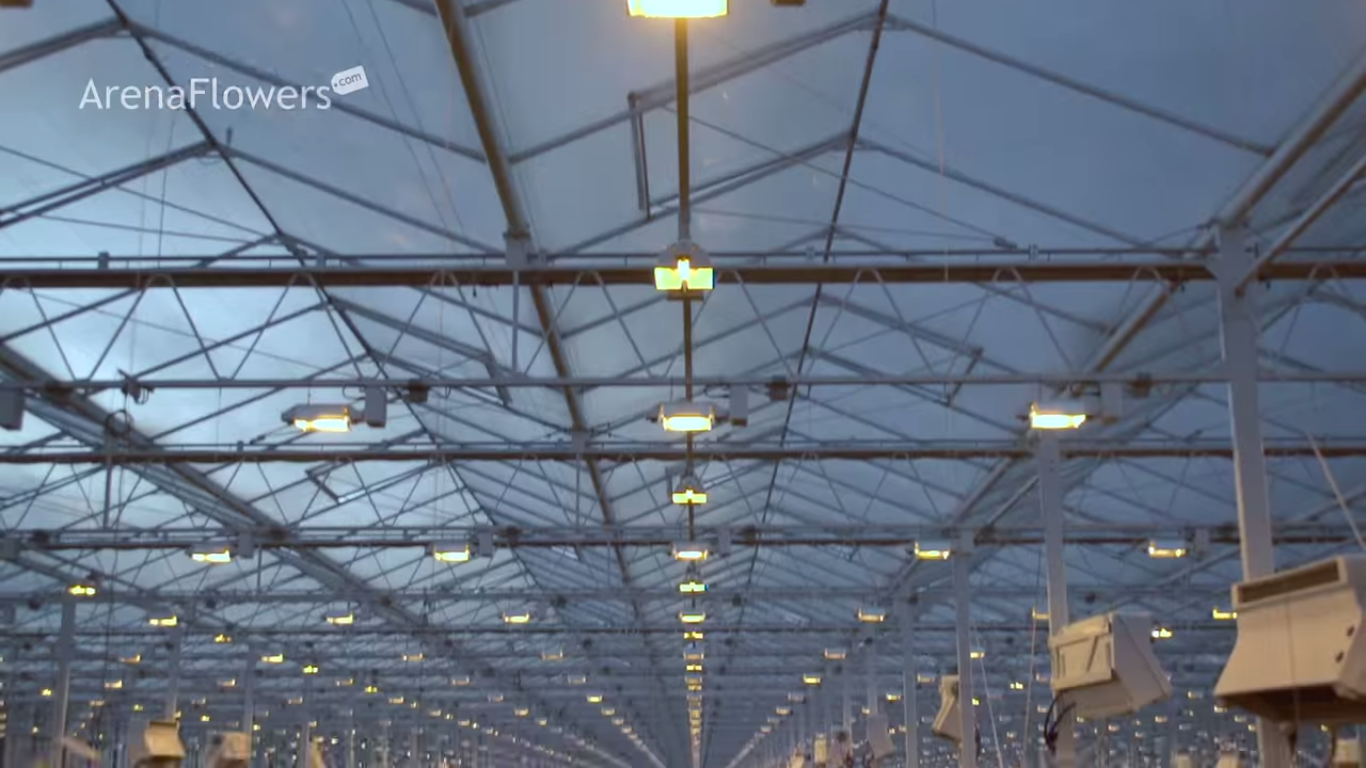
\includegraphics[width = 0.8\textwidth]{images/arena-light.png}
\caption{Arena Flowers Lighting}

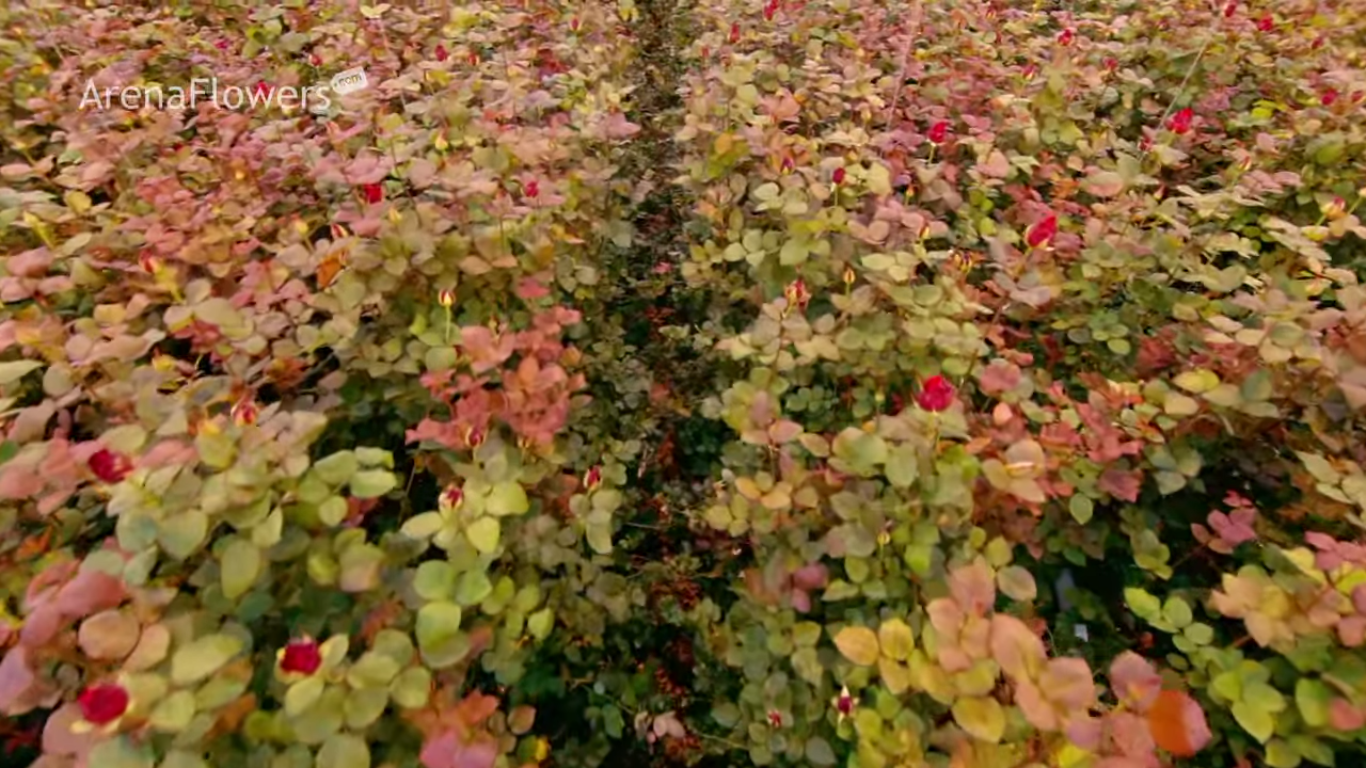
\includegraphics[width=0.8\textwidth]{images/arena-flower.png}
\caption{Arena Flowers}
\end{figure}

\begin{figure}[ht]
\centering
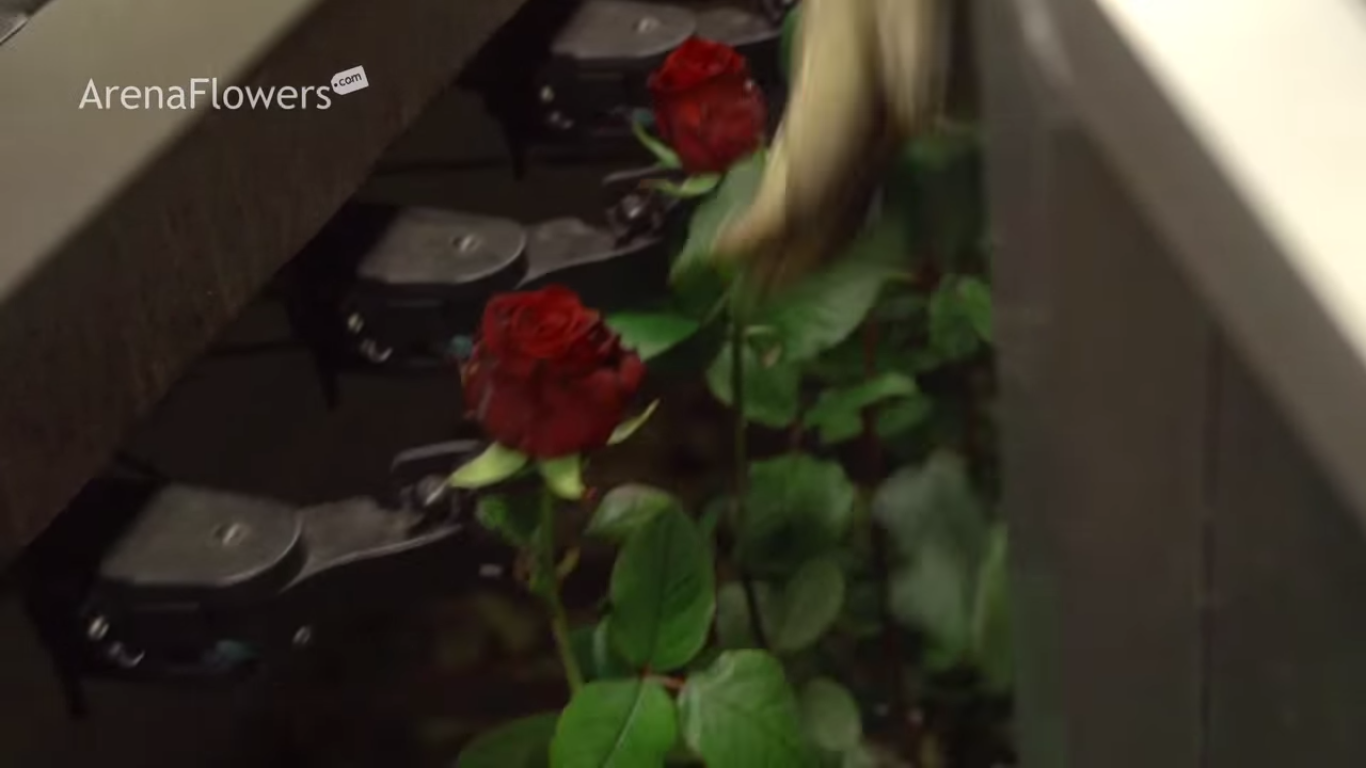
\includegraphics[width=0.9\textwidth]{images/arena-flower-selection.png}
\caption{Arena Flower Selection}

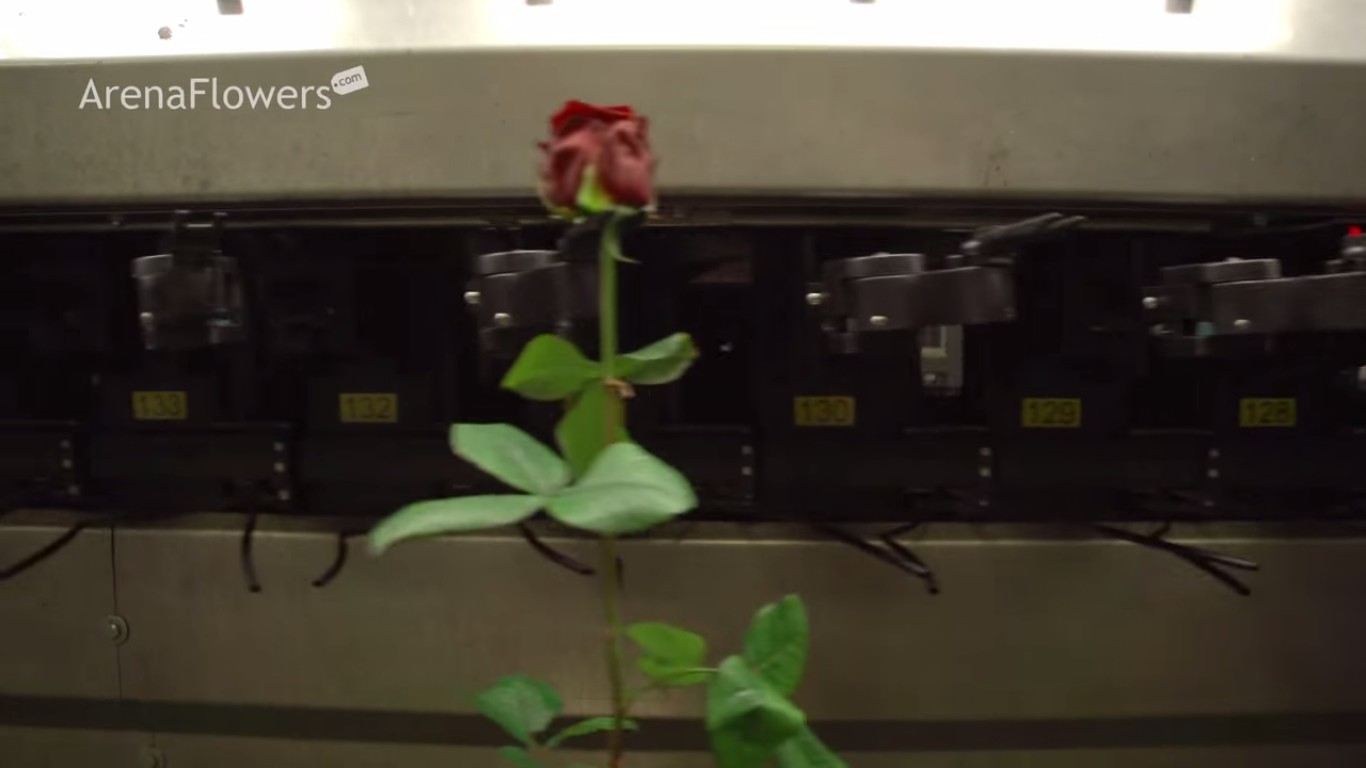
\includegraphics[width=0.9\textwidth]{images/arena-flower-selection-1.png}
\caption{Arena Flower Selection}
\end{figure}

\begin{figure}[ht]
\centering
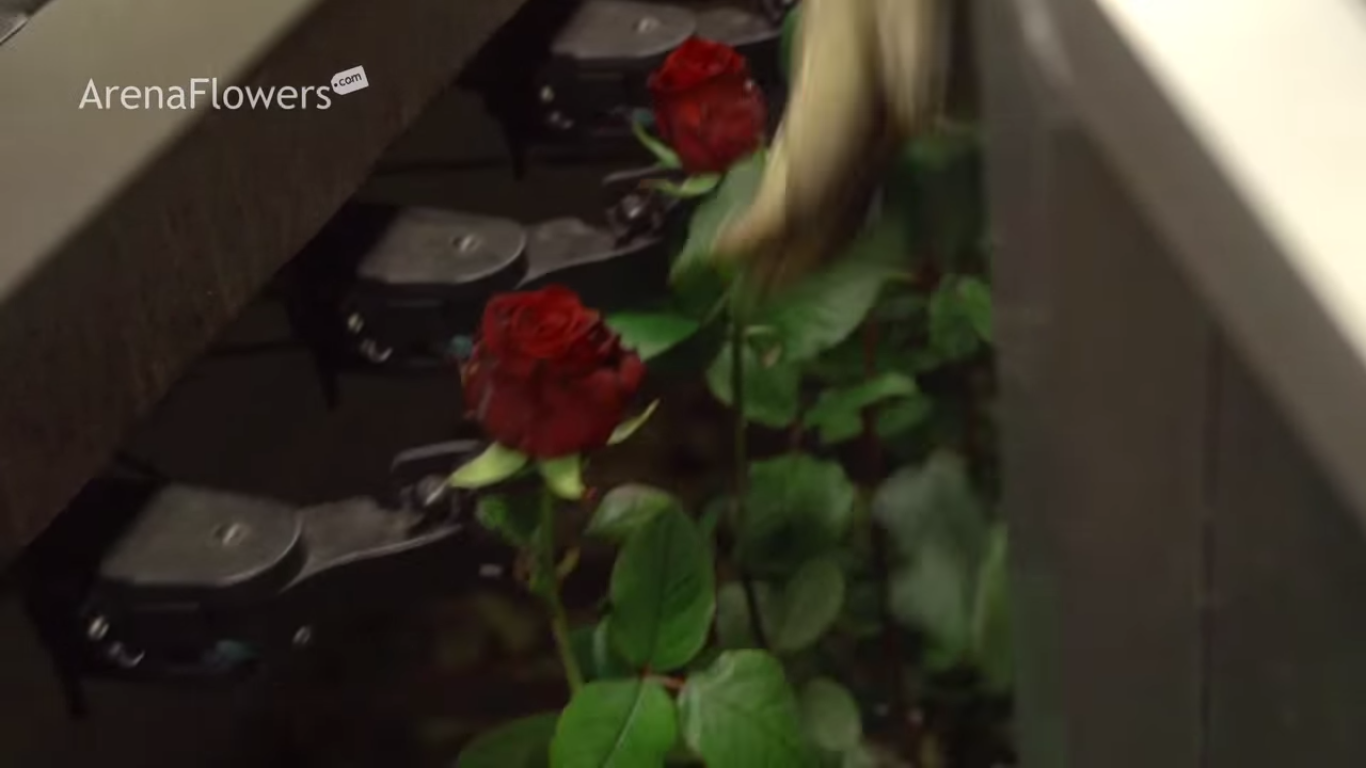
\includegraphics[width=0.9\textwidth]{images/arena-flower-selection.png}
\caption{Arena Flower Selection}

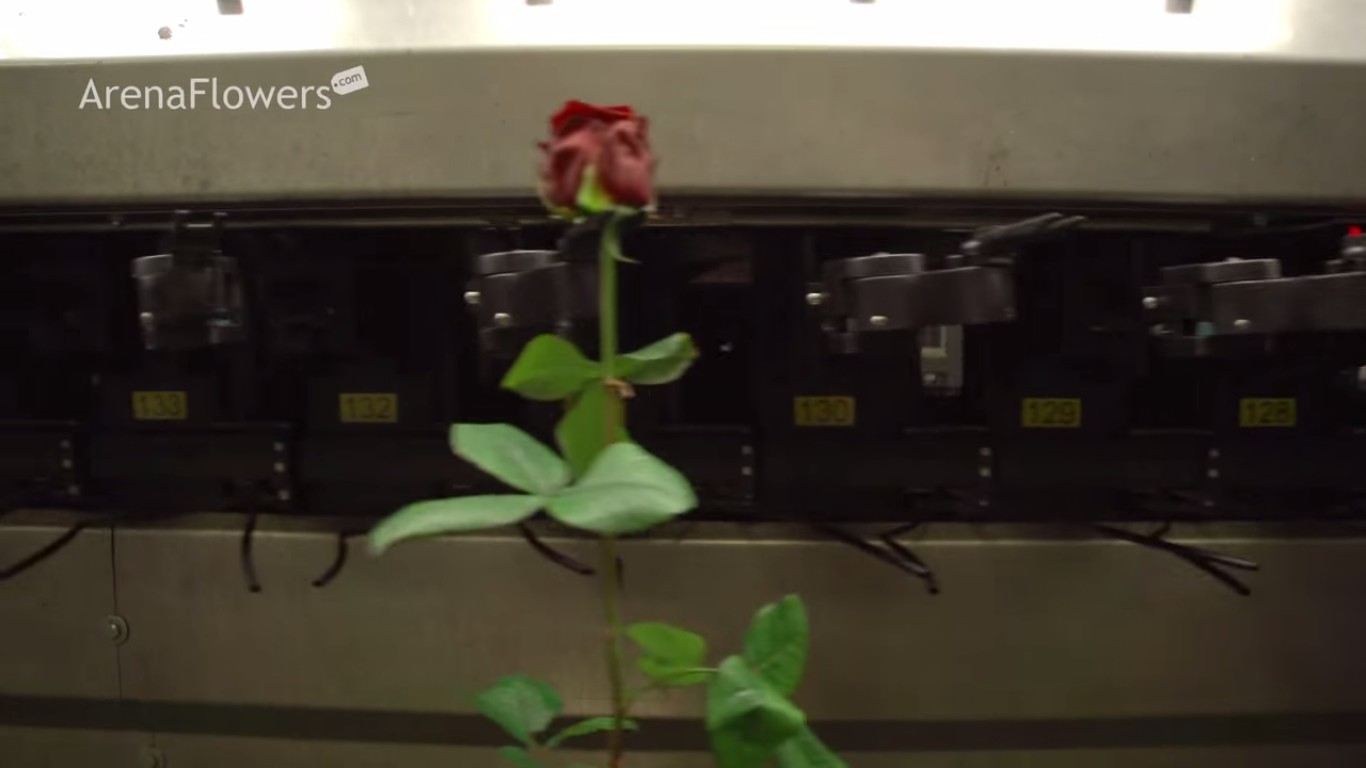
\includegraphics[width=0.9\textwidth]{images/arena-flower-selection-1.png}
\caption{Arena Flower Selection}
\end{figure}



\begin{multicols}{2}
\section{Emergency Assistance}
The biggest issue with quad-copter is battery life which is very poor at the moment. There has been proposal to enable solar charging while its on the air but that will need sophisticated hardware breakthroughs in battery technology and solar cells in particular before it can viable. The other issue is battery charging time which is time consuming and very slow.

A practical solution that has been suggested before is charging towers but it means a considerable budget for the infrastructure. The need arises for more practical solutions. If we look around and notice some of the biggest apps like \textit{`Uber'}, it solves the issue of transport in a resourceful manner. Instead of building new underpass, flyovers , subway stations, increased taxis; it provides an innovative and smart solution for the problem of \textit{`transportation'} by finding out the available \underline{resources} and \underline{demand} and running smart algorithms to cater the demand. 


Similarly, a smart solution to the problem of battery life is see the available resources. In cities there are power plants that are generating electricity for the masses, while in the remote areas there are communication towers and power grid lines. These are available resource that exist. So designing an electronic hardware that can utilize power from grids, communication tower and the likes for charging their batteries is a good idea.

The other challenge is charging time. There are several ways this can be tackled that will be elaborated later:
\begin{itemize}
\item A mechanism to switch the battery.
\item A set number of drone inside a cell to make sure continious availability of \textit{`charged'} quadcopter. 
\end{itemize}


\end{multicols}




\section{Health Management}
There are many patients who suffer from chronic disorder and they must visit the doctor regularly after every two months.

\begin{multicols}{2}
\subsection{Health Management}
There are many patients who suffer from chronic disorder and they must visit the doctor regularly after every two months.

\end{multicols}


\section{Java}
\paragraph{Buffered Reader}
To read characters from a text file, the FileReader is used. This reads bytes from a text file, and each byte is a single character. You can read whole lines of text, rather than single characters. To do this, you can hand your FileReader over to something called a BufferedReader. The BufferedReader has a handy method called ReadLine. As its name suggests, it is used to read whole lines, rather than single characters. What the BufferedReader does, though, is to store characters in memory (the buffer) so that they can be manipulated more easily.

\paragraph{} The BufferedReader is handed the FileReader object between its round brackets. All the characters from the file are then held in memory waiting to be manipulated. They are held under the variable name textReader.
The textReader object we set up is holding all the characters from the text file in memory (the buffer). We can use the readLine method to read a complete line from the buffer. After the line is read, we store the line in an array position.
The close method flushes the temporary memory buffer called \textit{textReader}. 

\begin{quotation}
while ( ( aLine = bf.readLine( ) ) != null )
\end{quotation}
Read each line of text and stop when a null value is reached." (If there's no more lines in a text file, Java returns a value of null.) Inside the curly brackets, we increment a counter called numberOfLines.




\section{Android}
\subsection{Debug}
\begin{quote}
Error during Sync: timeout when deploying apk to device 
\end{quote}
I faced this problem in eclipse and it was because of ADB connection timeout.
default was 5000 ms and it got fixed after changing that to 10000. \cite{captain}
	
	
\section{DALI}	

\begin{quotation}
This paper discusses the technology that allows user to control lighting in various possible scenarios. We will discuss how it is implemented in NMC Specialty Hospital.
\end{quotation}

\subsection{Introduction}
``DALI is a protocol, in which DALI devices communicate with each other" \cite{dali}. In simple words its a language just like HTTP where the DALI devices understand what is requested of them and how to send back requested information, what information to send when to simply turn on a specific light and what to make of any information that comes to any DALI device.

It is different than previous protocol is that in this system each lighting ballast can be addressed separately. 



\subsection{DALI Structure}
DALI consists of the following main elements:
\begin{itemize}
\item DALI Power Supply
\item DALI Controllers
\item DALI Data Cable
\item DALI Signal 
\item DALI Load Interface
\end{itemize}

\begin{center}
\begin{figure}[ht]
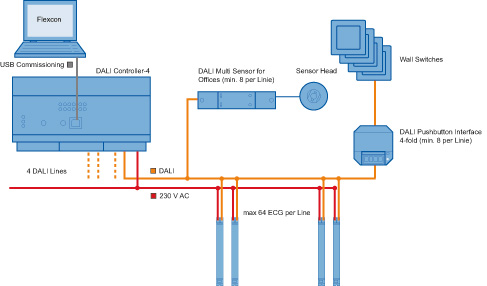
\includegraphics[width = 0.6\textwidth]{images/flexicon.jpg}
\caption{Flexicon DALI System Diagram}
\end{figure}
\end{center}

Notice the DALI Controller is taking inputs from Laptop, Sensor, Push Button Interface to control the amount of mains power that is allowed to the lighting ballasts.

\subsubsection{DALI Power Supply(DALI PSU)}
DALI Power Supply is responsible for creating the signal.

By default, DALI Power Supply maintains a potential difference of 16V across the wire and when button is pressed, the DALI power supply makes the circuit short and open by turn to generate a series of high(16V) and low(0V). Hence, a signal is generated without the need of any server computer or a processor.

\subsection{DALI Topology vs IP Topology}
This system should be easy to understand for those who are mildly familiar with IP networks. In DALI Network, the lights ballasts are connected in network, so that when a signal is sent to a particular ballasts, a switch connects the live wire to the neutral. 

It behaves in a similar fashion as that of IP network in the following ways:
\begin{itemize}
\item Devices are connected in a network that can have a certain topology.
\item Controllers are connected to Dimmers
\end{itemize}
There are many similarities 
A DALI network is similar to the regular IP networks that we are used to see in University Computer Lab and University Library. In place of computers, it has Lighting Ballasts.


\subsection{DALI Signal}
DALI control cable consists of 2 wires. The power supply creates +/- 16V potential between those wires. By short circuiting, the potential between the wires changes to 0V. By changing the voltage between 0V and 16V a digital signal is created.

The DALI signal consists of two parts, a ``where to'' and an ``info'' byte.


\begin{figure}[ht]
\centering
\begin{minipage}[b]{0.45\linewidth}
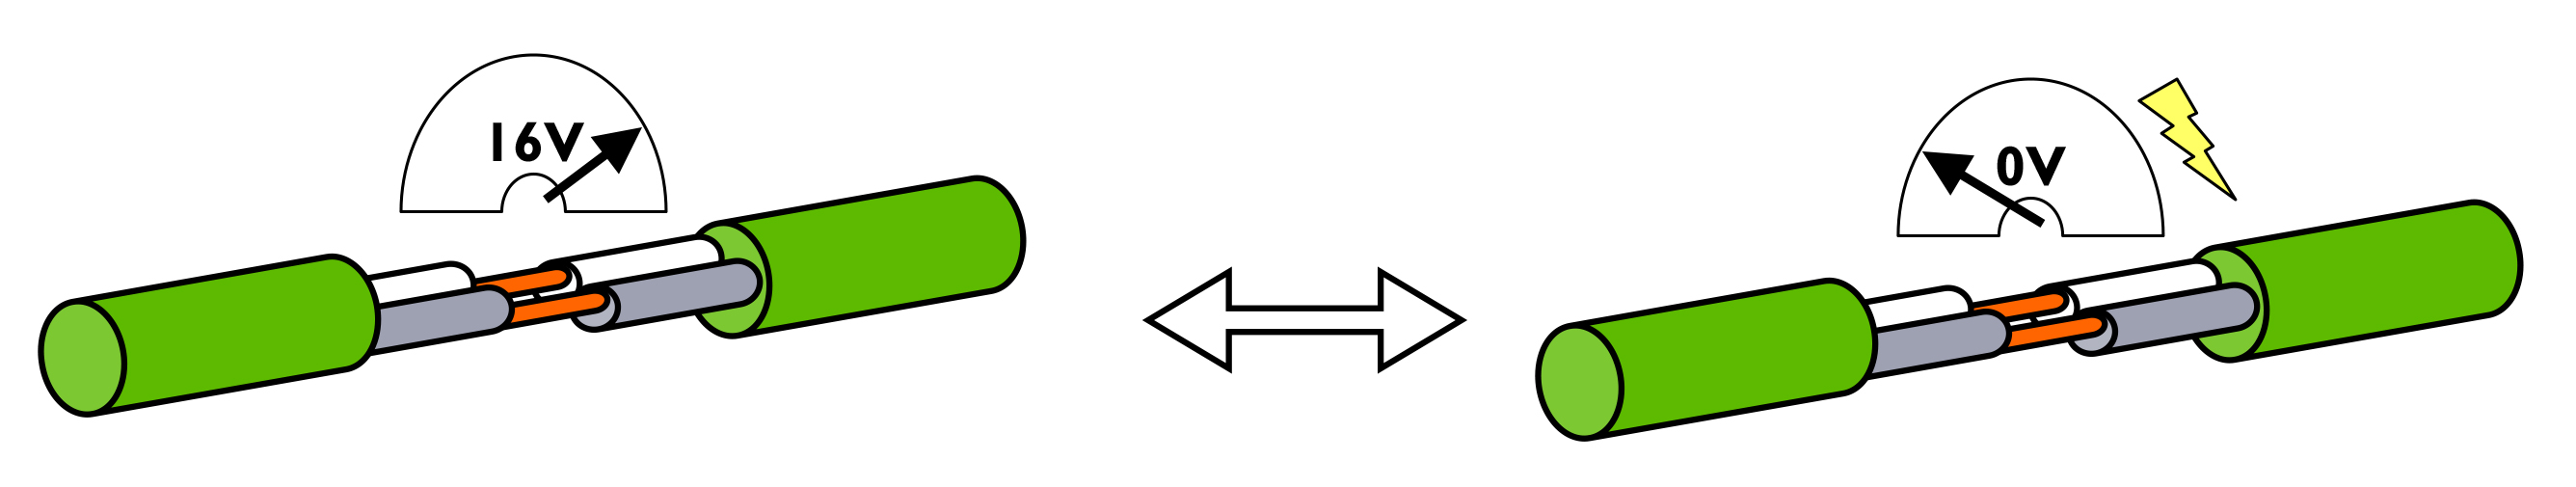
\includegraphics[width= 0.9\textwidth]{images/datacable.jpg}
\caption{DALI Data Cable}
\end{minipage}
\quad
\begin{minipage}[b]{0.45\linewidth}
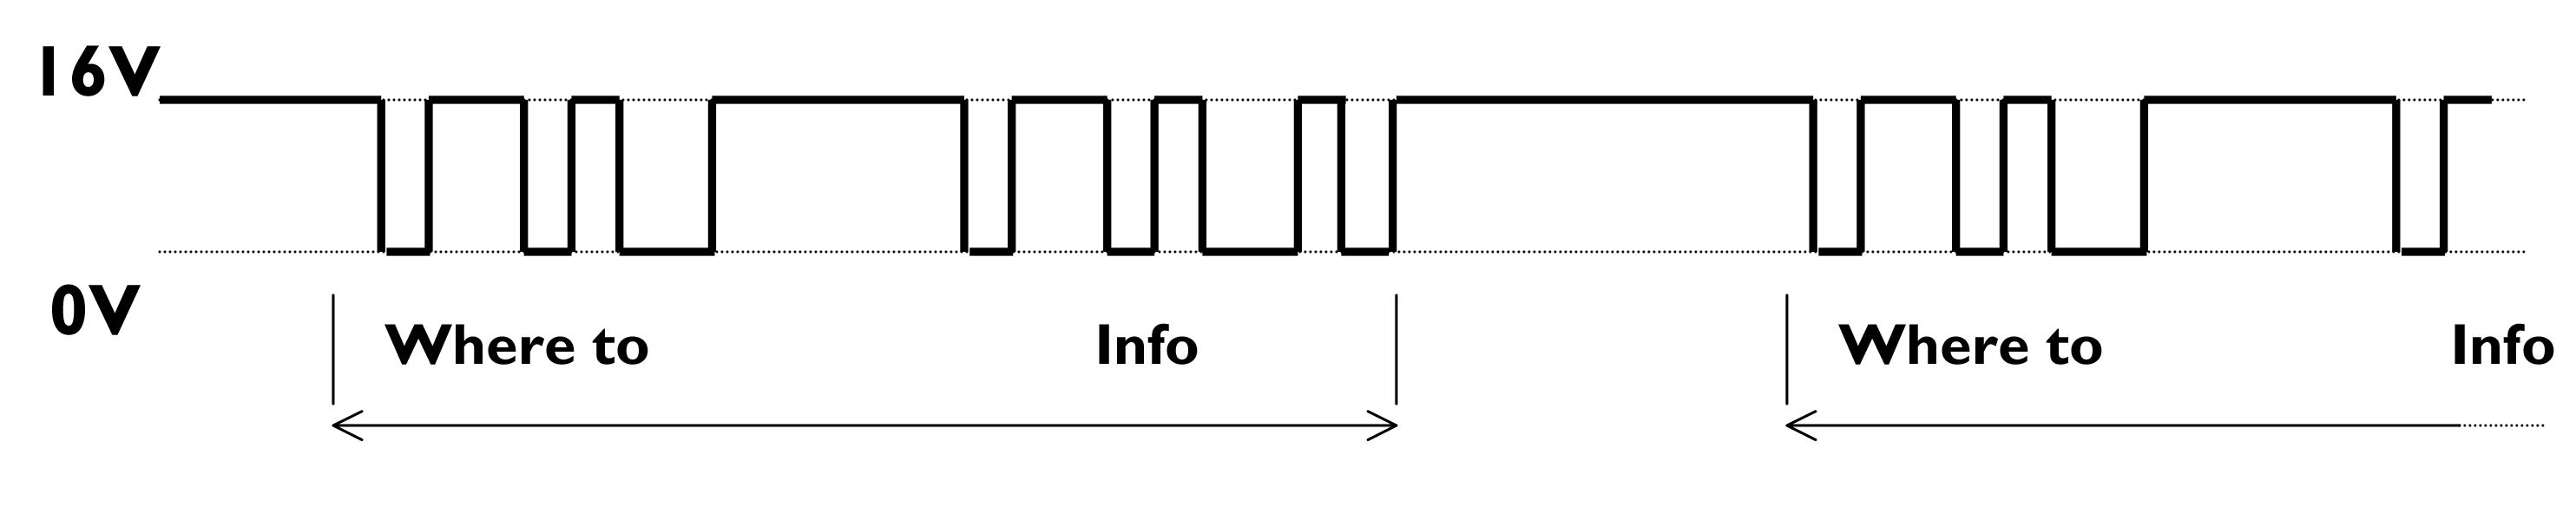
\includegraphics[width = 0.9\textwidth]{images/signal.jpg}
\caption{DALI Signal}
\label{fig:minipage2}
\end{minipage}
\end{figure}


The ``where to'' byte determines which devices should react.
\begin{center}
\begin{tabular}{|l|p{0.5\textwidth}|}
\hline 
\textbf{``\textit{where to byte}''} & \textbf{meaning} \\ \hline
Broadcast 		& all load interface will react \\ \hline
Group (1-16) 	& Load interfaces assigned to this group reach \\ \hline
Address (1-64)	& Load interfaces with this address react \\ \hline

\end{tabular}
\end{center}

The `info' byte determines what the device should do.
\begin{center}
\begin{tabular}{|l|p{0.5\textwidth}|}
\hline
\textbf{``\textit{info byte}''} & \textbf{meaning} \\ \hline
on 					& 	turn the lighting ballast on \\ \hline
off 				&	turn the lighting ballast off \\ \hline
direct level 50\%	& 	allow the exact amount of power from the mains in the ballast to make the light 50\% bright \\ \hline
step down 			&  	perform the step down scene \\ \hline
step up 			& 	perform the step up scene \\ \hline
recall scene 2 		& 	scenes are usually pre-configured brightness level \\ \hline

\end{tabular}
\end{center}

\subsection{DALI Controller Information}
A DALI controller will always be assigned a combination of ``where to'' and ``info'' information.


\begin{figure}[ht]
\centering
\begin{minipage}[b]{0.45\linewidth}
\begin{tabular}{|l|p{0.5\textwidth}|}
\hline
\textbf{``\textit{info byte}''} & \textbf{meaning} \\ \hline
on 					& 	turn the lighting ballast on \\ \hline
off 				&	turn the lighting ballast off \\ \hline
direct level 50\%	& 	allow the exact amount of power from the mains in the ballast to make the light 50\% bright \\ \hline
step down 			&  	perform the step down scene \\ \hline
step up 			& 	perform the step up scene \\ \hline
recall scene 2 		& 	scenes are usually pre-configured brightness level \\ \hline

\end{tabular}\end{minipage}
\quad
\begin{minipage}[b]{0.45\linewidth}
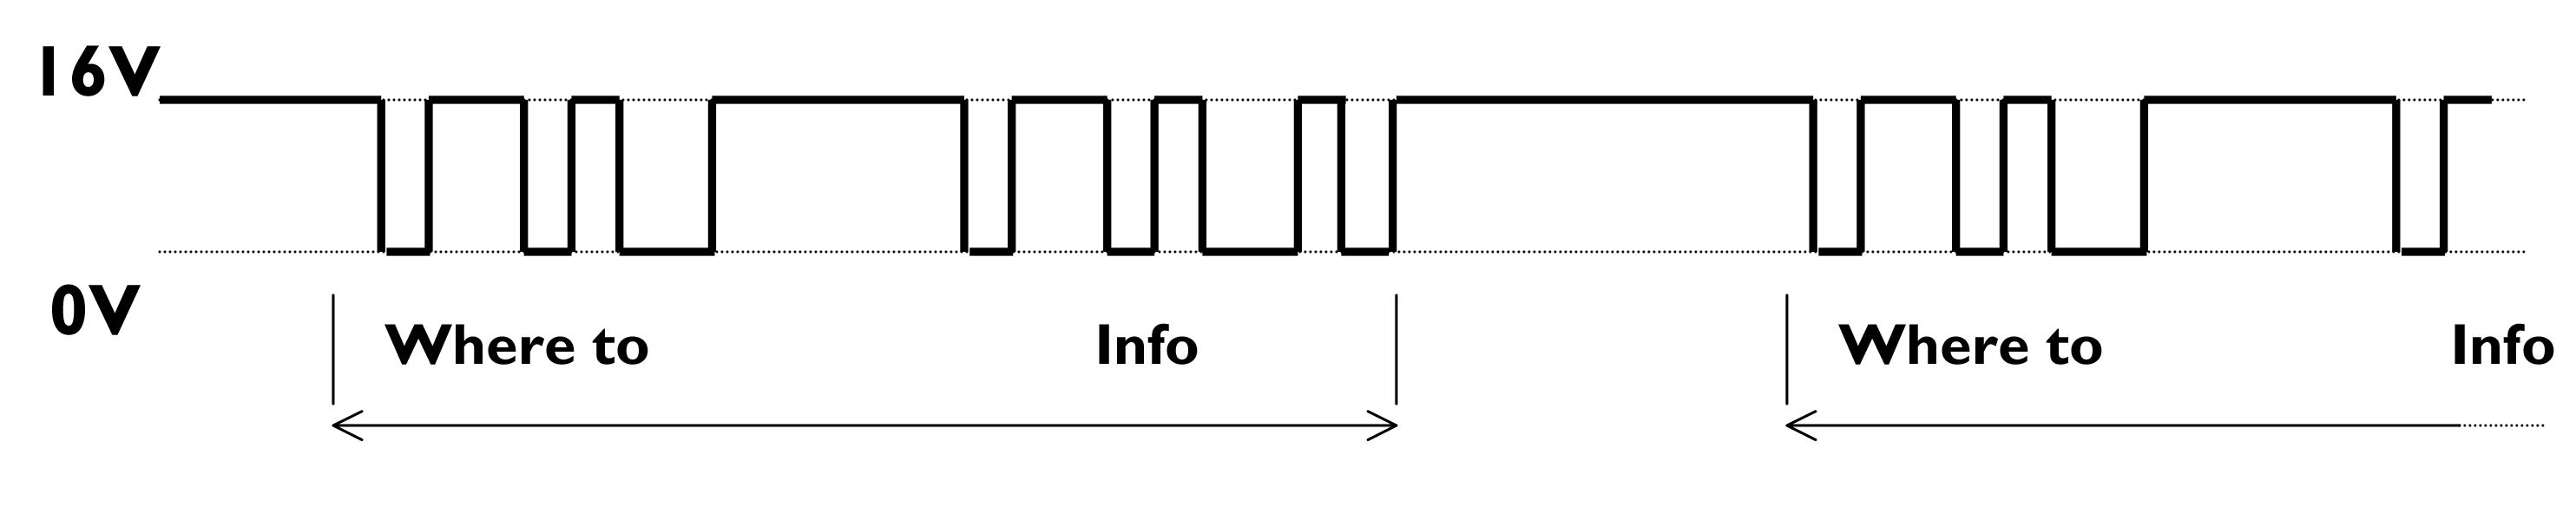
\includegraphics[width = 0.9\textwidth]{images/signal.jpg}
\caption{DALI Signal}
\label{fig:minipage2}
\end{minipage}
\end{figure}

\begin{figure}[h]
\centering
\begin{minipage}[b]{0.45\linewidth}
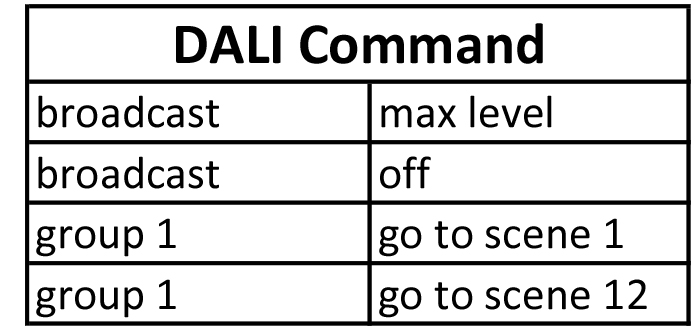
\includegraphics[width= 0.9\textwidth]{images/dalicommand.jpg}
\caption{DALI Command}
\end{minipage}
\quad
\begin{minipage}[b]{0.45\linewidth}
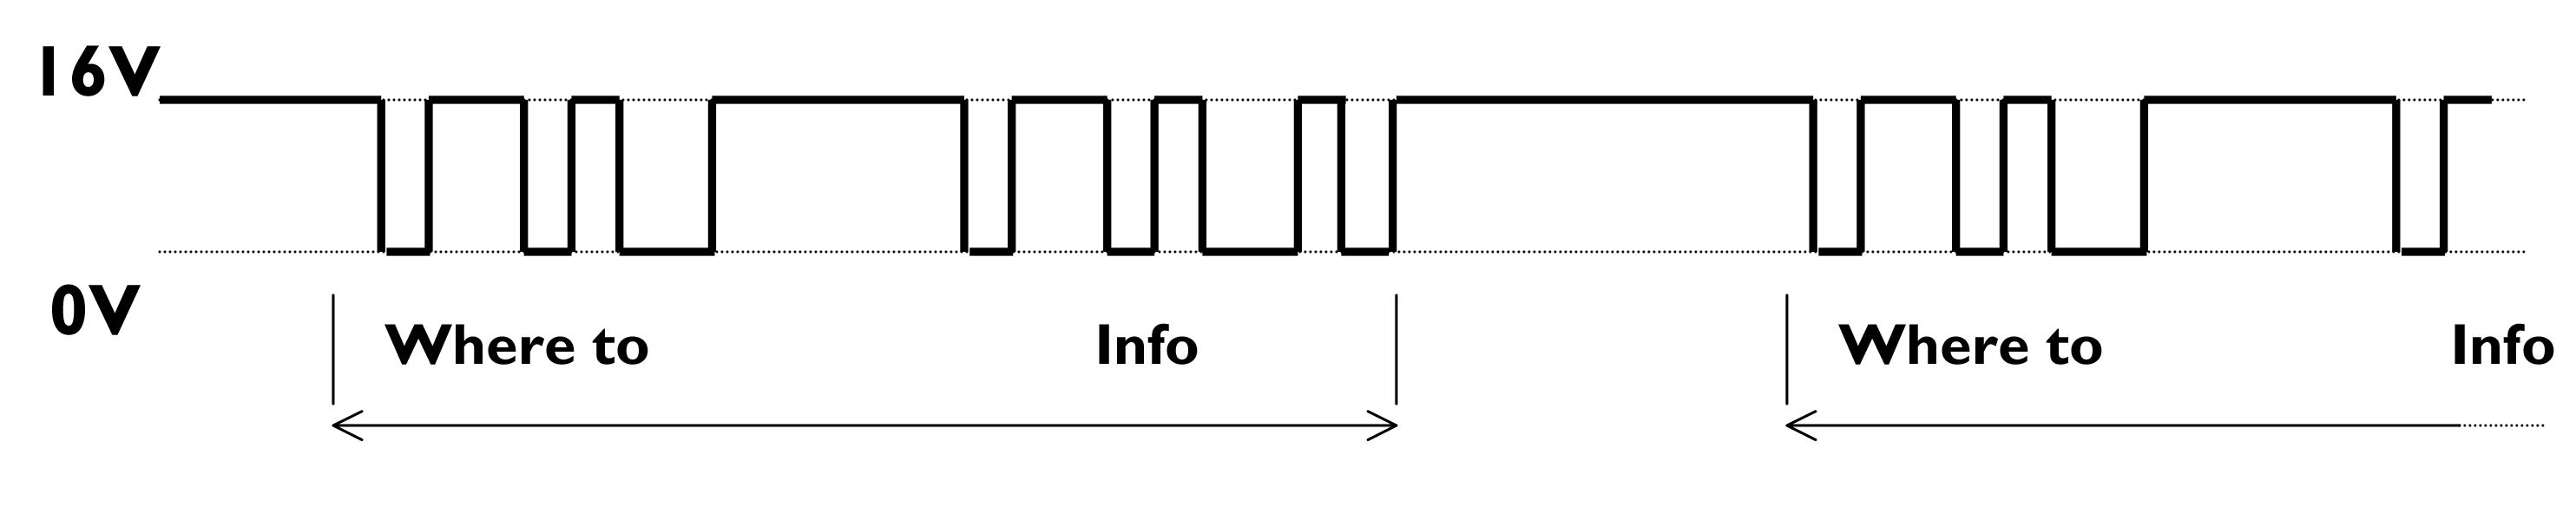
\includegraphics[width = 0.9\textwidth]{images/signal.jpg}
\caption{DALI Signal}
\label{fig:minipage2}
\end{minipage}
\end{figure}


\subsection{DALI Load Interface Identification}
For identification of the Load Interface they are:
\begin{itemize}
\item assigned a ``short address'' (1-16)
\item assigned to one or more ``groups''
\end{itemize}

\begin{figure}[h]
\centering
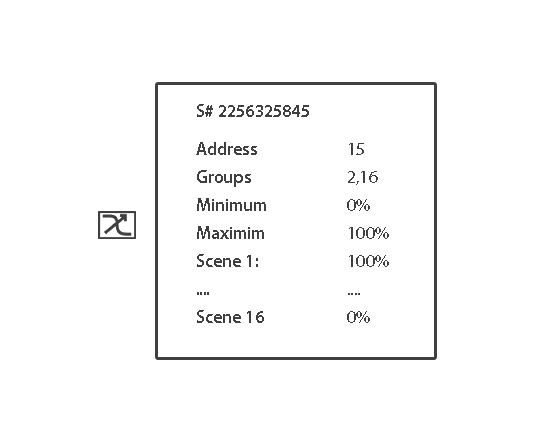
\includegraphics[width = 0.5\textwidth]{images/loadinterfaceinformation.png}
\caption{Load Interface Information}
\end{figure}

To obtain required intensity behavior of the Load Interfaces, they are also assigned:
\begin{itemize}
\item Intensity values for scenes
\item Minimum Intensity value
\item Maximum Intensity value
\item Fading time (0s - 1.5m)
\end{itemize}

\begin{figure}[h]
\centering
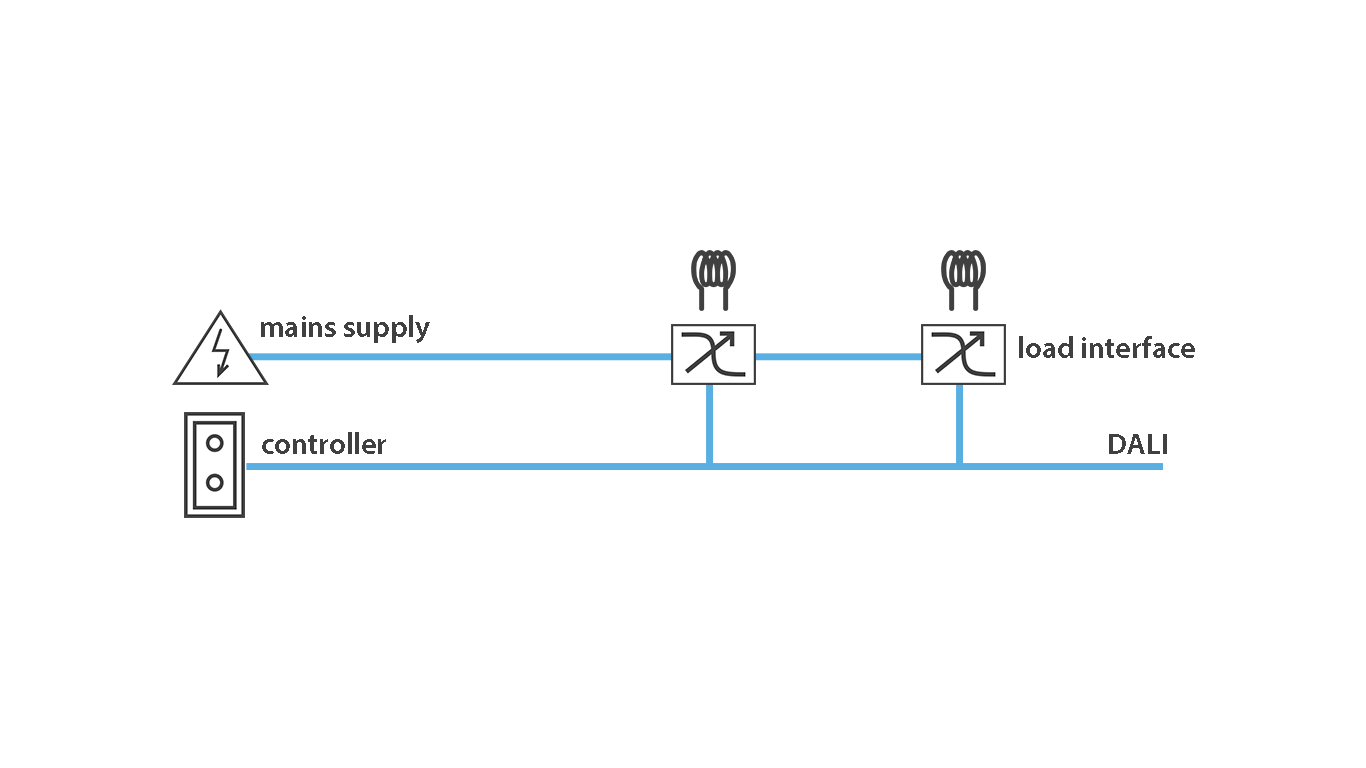
\includegraphics[width = 0.8\textwidth]{images/system.png}
\caption{DALI System Diagram}
\end{figure}

\subsection{DALI Topology}
Topology with DALI is free; serial, parallel, combination. The total DALI length should be less than 300m.

\subsection{DALI Power Supply}
The power needed for the DALI-signal can be created by an external power supply. Some products have the functionality of DALI power supply integrated; i.e MultiDim Dimmers.

Note: Always use exactly `1' power supply in a DALI System.

\subsection{DALI Technical Characteristics}
\begin{itemize}
\item Communication is always started by the controller
\end{itemize}

\subsection{DALI Transport}
DALI requires 2 wires to a device, in addition to mains cable if required. These wires are not polarity dependent which makes it simple to install. These wires are ELV(Extra Low Voltage) potential and are looped to all devices. Some devices, such as HF Ballasts are mains powered, and only have functional isolation between the mains and the DALI Control. This means that even though the DALI control cable operates at ELV potential, it must be treated as if at mains supply.

A DALI network requires a 24V DC 250 mA power supply to operate. This voltage appears on the data cables and can be used to supply power to peripherals that require it; such as motion detectors. A separate power supply can be used, some manufactures have DALI gateway with integral power supply.

When choosing DALI Cable, use a mains rated cable with conductor size as per chart below:

\begin{tabular}{|l|l|}
\hline
\textbf{Length} & \textbf{Conductor Size} \\ \hline
< 150 m & 0.5mm\textsuperscript{2} \\ \hline
100 m - 150 m & 0.75 mm \textsuperscript{2} \\ \hline
> 150 m & 1.5 mm \textsuperscript{2} \\ \hline
> 300 m & Not recommended \\ \hline
\end{tabular}

\subsection{Dimmable HF Ballast Control Comparison}
\begin{tabular}{|p{0.12\textwidth}|p{0.12\textwidth}|p{0.12\textwidth}|p{0.12\textwidth}|p{0.12\textwidth}|p{0.12\textwidth}|}

\hline

\textbf{Control Type}	& \textbf{Control Cable}	& \textbf{Control Signal}	&\textbf{Polarity}	&\textbf{Individually Addressable} & \textbf{0\% while Energised}  \\ \hline
DALI & 2 wire & Manchested Encoded & No & Yes & Yes \\ \hline
DSI &  2 wire & Manchested Enchoded & No & No & Yes \\ \hline
1-10V & 2 wire & 1-10V DC Analogue & Yes & No & No \\ \hline

\end{tabular}

\subsection{DALI Companies and Services}
There are various companies that manufacture DALI Devices and following is a list of manufactures:

\begin{tabular}{|l|l|}
\hline
\textbf{Product} & \textbf{Company} \\ \hline
\href{http://www.osram.com/osram_com/news-and-knowledge/light-management-installation-made-easy/installing-light-management-in-commercial-enterprises/index.jsp}{DALI Professional} & OSRAM \\ \hline
\end{tabular}

\subsection{DALI Devices Power Consumption}
DALI devices consume power to operate. DALI ballasts have the capability to fully extinguish the lamp with mains power still applied to the ballasts.This can simplify the mains wiring of some implementations as there is no requirements to switch off the mains when the lights are turned off.

\subsection{Dimming Curve}
The DALI protocol provides 256 levels of brightness between off and 100\%, which is translated to ballast power level via a logarithmic dimming curve. This curve gives larger increment in brightness at high dim levels and smaller increment at low dim levels. This is an attempt to have a dimming curve which appears linear to the human eye.


% ---------------------------------
% ------ Something in Air ---------
% ---------------------------------
\section{Reduced Usage of Pesticide}
The aim of the researches is to reduce the use of pesticide and find healthy alternative to combat the damage done by pesticide. Pest is a big concern for farmers specially for greenhouse farmers. They have the potential of damaging crops in massive scale and incur big financial loss. The challenge faced by farmers are that they are unable to detect the time when a crop is inflicted with pests and hence they spray pests over the whole crop in advance in case they are attacked by pests.

\section{Grey Mould}
\textit{Botrytis cinera} is a fungus that grows and thrives in cool and wet conditions and establishes itself on dying tissues. It produces masses of dry spores called conidia that are airborne. If the right conditions are given it can cause epidemic. It has a list of different hosts including tomato, pepper and lettuce. It can infect almost all part of a plant, including stem, leaf, peduncle and fruit. It begins with leaf-pruning scars and peduncles(fruit stem) often leads to stem canker which is the most destructive stage of the disease causing substantial crop losses.

\begin{figure}
\centering
\begin{minipage}[b]{0.45\linewidth}
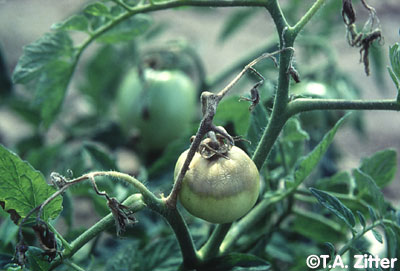
\includegraphics[width=0.8\textwidth]{images/botrytis-mold.jpg}
\caption{Gray, velvety covering of spores of Botrytis cinera develop on dying flowers and lead to subsequent infection of fruit.}
\end{minipage}
\quad
\begin{minipage}[b]{0.45\linewidth}
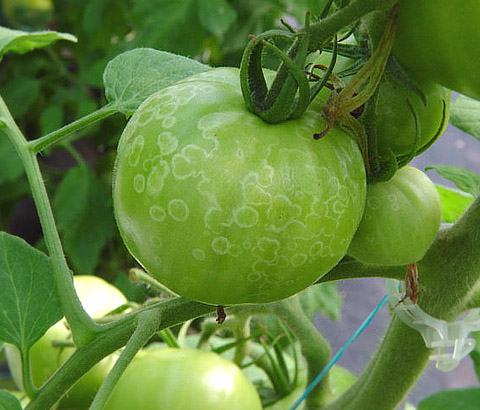
\includegraphics[width = 0.8\textwidth]{images/botrytis-ghost.jpg}
\caption{Botrytis ghost spots on greenhouse tomato fruit}
\end{minipage}
\end{figure}


% ---------------------------------
% ---- Power Management System-----
% ---------------------------------

\clearpage
\section{Smart Load Management System}
This paper attempts to illustrate the whole concept of \textit{\textbf{Power Management System}} through illustration and diagrams.

\subsection{Power Management System}
\begin{figure}[h]
\centering
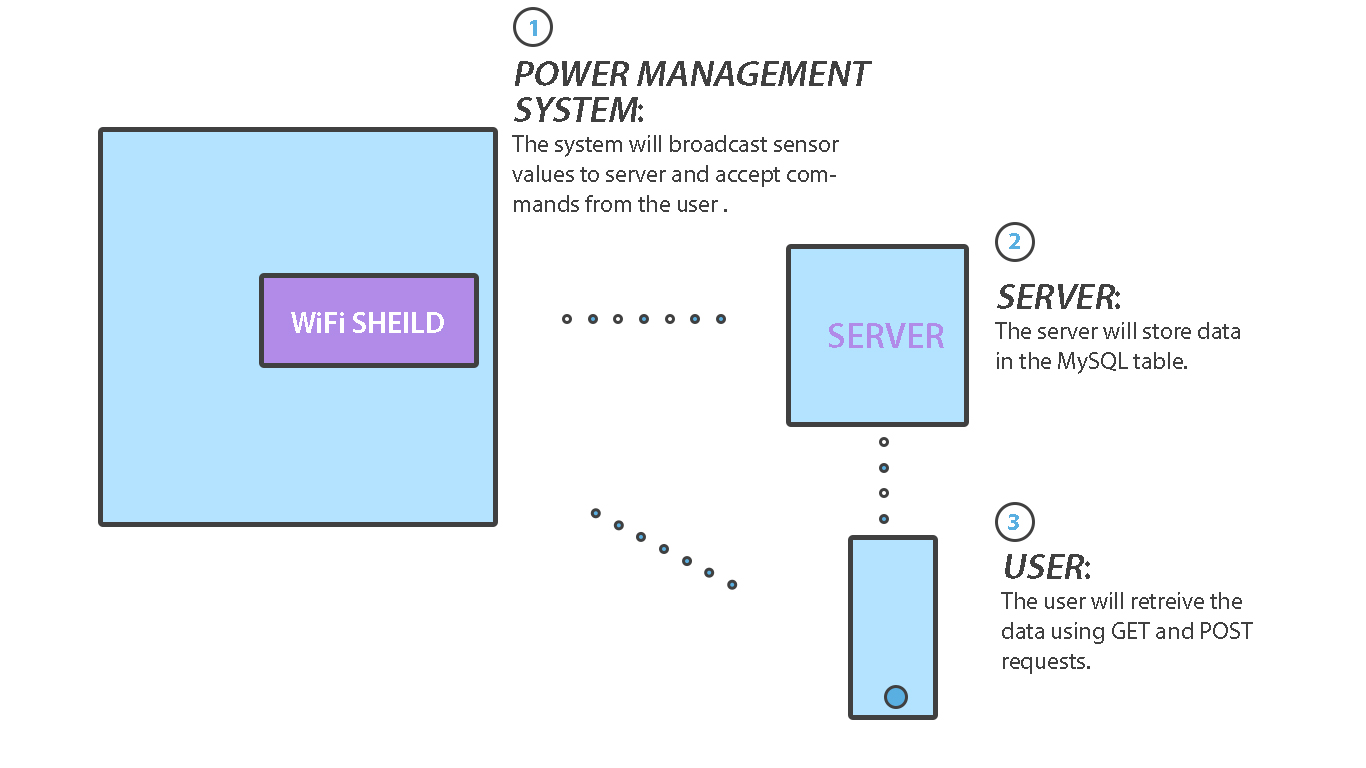
\includegraphics[width = 0.6\textwidth]{images/PowerManagement.jpg}
\caption{An Overview of the Power Management System}
\end{figure}

\begin{figure}[h]
\centering
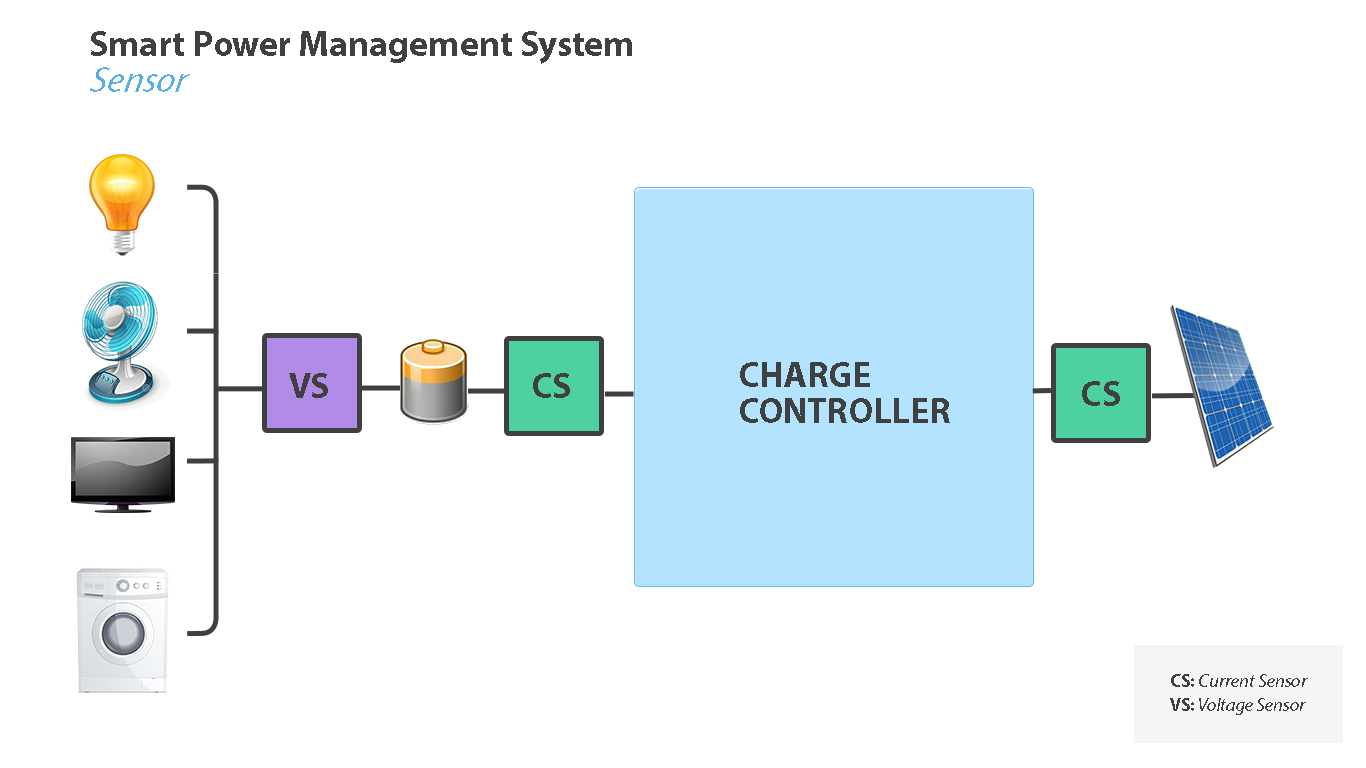
\includegraphics[width = 0.6\textwidth]{images/PowerManagementSensor.jpg}
\caption{An Overview of the Sensors Involved in Power Management System}
\end{figure}


\begin{figure}[h]
\centering
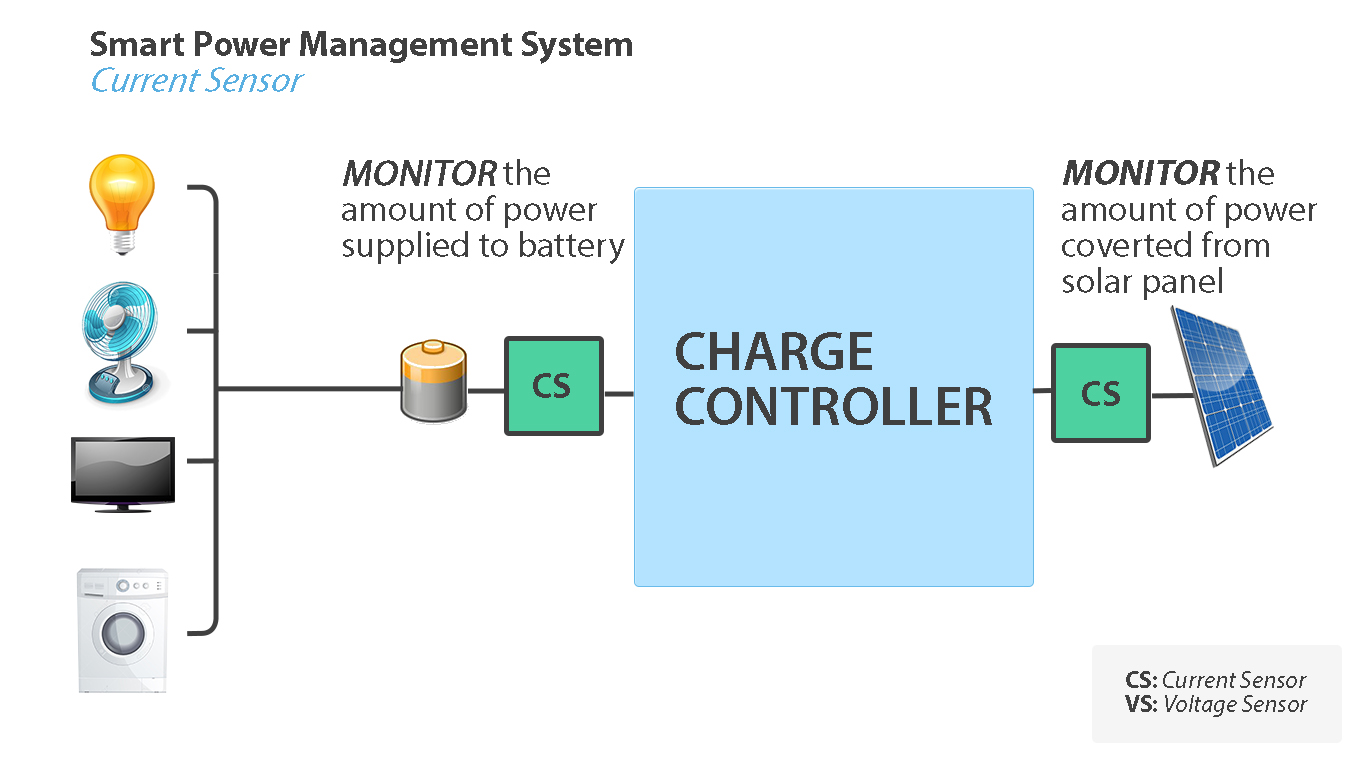
\includegraphics[width = 0.6\textwidth]{images/PowerManagementCurrentSensor.jpg}
\caption{An Overview of the Sensors Involved in Power Management System}
\end{figure}

\section{Investigation of Load Side Monitoring Methodology}
\begin{multicols}{2}

We wanted to today was to monitor the currents and through the current ultimately the power consumed by every AC load. We worked with an ACS712; a typical bulb, a battery and an inverter. However, there was some complication involved which had to do with the waveform of the ac. Unlike the DC which has a constant straight line voltage value. Also, the complication involved the rate of reading of analog values and the time it would take to take reading for a complete cycle. This is not constant, since with every line of code the clock speed changes; with every line the time of analog read varies as the chip has to go through an extra calculation which in turn takes up more time.

\paragraph{} In our investigation to measure the amount of steps to complete one cycle of 50 Hz AC, we carried out a study of the behavior of an atmega328p. A maximum sampling rate of an Atmega chip is 10,000 samples per second.\cite{arduinosamplerate}

\paragraph{} Considering the above stated facts and assumptions the plan of action is to acquire a series of readings of ADC values that correspond to the AC current (I rms) values. We attempt to find a symmetrical pattern in the readings that hint to the zero-crossings of the waveform. We then use our intuition to sketch a rough graph of the AC current with the displayed ADC values and from here we will know the number of ADC steps to complete one AC cycle. Once we know that, we do a series of small calculations to convert this current into RMS current which will then be displayed on the serial monitor. 


\end{multicols}








% -----------------------
% ---- Bibliography -----
% -----------------------

\clearpage
\bibliographystyle{IEEEtran}

\begin{thebibliography}{100} 

\bibitem{arduinosamplerate} \textit{Arduino Getting Started} Arduino. Available: \url{http://arduino.cc/en/Reference/analogRead}

\bibitem{leicester} \textit{Concrete topics for PhD research} Ruzanna Chitchyan. Available: \url{http://www2.le.ac.uk/departments/computer-science/postgraduate/research/topics}

\bibitem{captain} \textit{Error during Sync: timeout when deploying apk to device using maven}. Captain Overflow. 

\bibitem{greenhousewatering} \textit{Energy use, greenhouse gas emissions, and water use in Canada, 2011}. Available: \url{http://www.statcan.gc.ca/daily-quotidien/150126/t150126a002-eng.htm#note_2}

\bibitem{dali} \textit{Introduction to DALI} Philips. Available: \url{http://www.dte.us.es/docencia/etsii/itis/emc/Transparencias/domoinmo/dl} [2008].

\bibitem{advantage}\textit{Free Space Optics Advantages and Disadvantages }” Outdoor Wireless Communications . Available: \url{http://www.fso.net/advantages-disadvantages.html} [2013].

\bibitem{challenges}\textit{Hybrid Free-Space Optical and Radio-Frequency
Communications: Outage Analysis}” ISIT University of Texas . Available \url{www.itr.unisa.edu.au/itrusers/nguyendk/.../Hybrid_FSO_RF_ISIT.pdf‎} [2010].

\end{thebibliography}



\end{document}
